\section{Aire Guru}

Urban residents are surrounded by many sources of air pollution, and it is the direct cause of many different symptoms,
ranging from simple eye irritation 
to, in extreme cases, death. Particularly for high-risk groups like children and the elderly.
The WHO (World Health Organization) estimates 4.2 million deaths
(https://www.who.int/
airpollution/ambient/en/) per year due to air pollution.
Air pollution has a significant affect on people with asthma, cardiopathies, allergies, and neurological pathologies.\\

Air pollution not only aggravates existing diseases, but can also be an initial cause of them, such as in the case of foetal brain
damage (https://www.cronicabalear.es/2018/07/la-contaminacion-ambiental-causa-enfermedades-neurologicas-y-envejecimiento-del-cerebro)
caused by the mother's exposure to air pollution.\\

To be able to control the level of exposure we need to know the levels
in the specific locations that we frequent, and the variation during specific times.
To make this information as accessible as possible, it should be freely and publicly available, and the presentation
must be simple enough to be understandable by the average citizen.\\


We have created a website - Aire Guru - which collects air pollution data periodically, stores it for historical use, 
processes it to extract relevant information, personalizes it to engage the user with regard to their individual
circumstance, visualizes it in an easy to understand format, and provides it online to facilitate its accessibility free of charge. Furthermore,
descriptions of all the data and how it has been processed are also provided to raise public awareness of the value
of this data. Aire Guru has been successfully tested, using the Air Quality data provided
by the Málaga open data portal(https://datosabiertos.malaga.eu/) in the Spanish city of Málaga.\\

There are already many tools available, however they have various failings.

The most common problems are:

\begin{itemize}

    \item Obsolete measurements. Measurements need to be taken regularly, since there can be huge differences
          between pollution levels at different times of the day.

    \item Limited geographic coverage. The data must cover a reasonable proportion of areas that people spend significant time in.

    \item Insufficiently granular measurements. Measurements must be at a reasonably fine level of granularity. One single measurement for an entire city is not useful.

    \item Poor presentation. Often the information is presented in an uninterpreted form, making it difficult for users to visualize, especially in a geographic sense.

    \item Poor discrimination and interpretation. Many tools show individual values as a number or a colour. This information is not
          enough for the user to take control of their exposure. Such visualizations are not really compelling. 

\end{itemize}

Our website solves the deficiencies described above.\\

Measurements are published hourly and come from measurement stations placed throughout the 
city of Málaga, covering entire urban region at a granularity of $100m^2$.\\

The information is presented in a clear and simple manner, making it possible to see the most polluted regions,
and allowing the user to make comparisons both geographically and historically. It provides personalised information, such as the most relevant 
pollutants for a user's particular medical conditions, and can track
the pollution they are exposed to both in real time and over a historical period, by linking with location data from their mobile device. \\

To achieve our goals we have fronted the following challenges:\\

As we mentioned it before, the data is provided on the Malaga's open data portal.This is not a intuitive place to search the
air pollution information for the averange user. Even if the user find it, it is not 
easierly located. Aire Guru needs to provide the information in a way that it is easier for the user and preferably, direct.
This means, Aire Guru shows the information without the need for the user to perform any extra action, just opening the
website in a browser.\\

The data offered in the open data portal is in GeoJson format. This format is highly structured and using specific software could be
processed i a relatively easy way, even though, it is not really interpretable for humans. Aire Guru translate all the 
data in usefull information in a format more understandable for the users, like graphs, icons, colors and text.\\

It also intruduce interactibity, making possible to navigate throuw the data.\\

Coming back to the data provided on the origin source, we should notice that each sample, measurements of an station, offers a different
set of fields. Aire Guru is able to proccess all of them and offer the user an unified vision of the measurements offered by
all the stations.\\

It also allow the user to visualize the pollution in an specific area in an specific time with the less amount of effort.
As we mention, the data is structured by mesuarement stations, the range of action is defined by the coordenates of 
a polygon. To be able to get this data, the user should manually interpolate a location with the polygons defined in the dataset.
This is not a really duable task if we would like to monitor the pollution around us or in an specific area. Aire guru
automatize all these proccess and offer an intuitive interface to perform theses actions.\\

We should notice that the data provided contain a set of values will help us to calculate the level of pullution. Aire guru
does this for us. It offers the values but it also offer the information, that means, if we are in a safe enviroment or not.\\

These data is not static, it is published every hour, so, to obtain the most updated value, Aire guru implements an structure
which allows it to obtein and represent the data with the same periodicity.

Malaga's air quality dataset is updated every hour, Aire Guru automates the process of collecting the
data through a CRON job that executes a script implemented in JavaScript periodically. This reads the data from the url, processes it,
cleans and stores it in a MongoDB database. That is to say, Aire Guru implements all the necessary collection processes.\\

Thanks to this infrastructure, the user is able to visualize the evolution of pollutants since 2018. The user can also track their personal exposure
 to these pollutants over the same period of time.\\

In addition, this automation allows the user to visualize the pollution in the city of Málaga in real time, and see specifically the location where he is 
occurring. \\

\begin{figure}[ht]
    \centering
    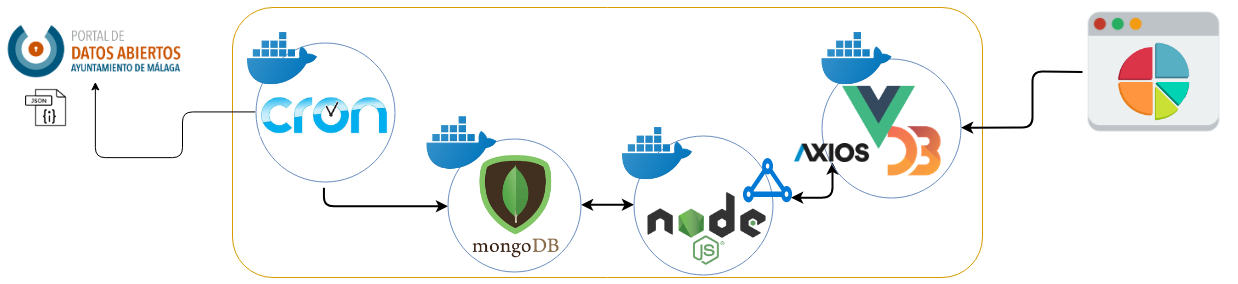
\includegraphics[width=12cm]{Figure_2_1_aireGuruArquitecture}
    \caption{Arquitecture Aire Guru}

\end{figure}

\begin{center}
\bf Figure 2.1. Arquitecture Aire Guru\\
\end{center}
The data to the users through a web interface. \\

\begin{figure}[ht]
    \centering
    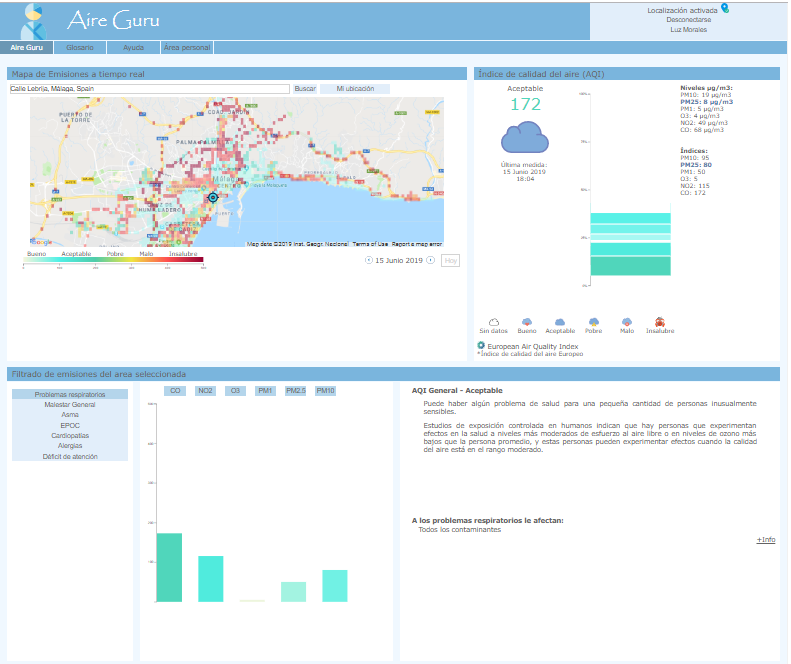
\includegraphics[width=9cm]{Figure_2_2_aireGuru_webInterface}
    \caption{Aire Guru. Web Interface}
\end{figure}
\begin{center}
    \bf Figure 2.2. Aire Guru. Web Interface\\
    \end{center}
To enable access by the majority of the population, Aire Guru is available at the web addresses https://www.aire.guru and https://www.airquality.guru.
We use SSL that guarantees the encryption of data through the network and ensure the user has access to it since, as more and more browsers try to protect 
users by only showing pages that use a secure method.\\

As we commented previously, all users can see the basic information without having to provide any data or identify themselves, without the need to
perform downloads or installations. Today, almost everyone is familiar with web browsing and if we do not force the user to realize extra taks, as 
requiring them to sign in or install extra software, the probability the user uses our platform will be higher. 

\subsection*{Evaluation}

The system has been successfully tested with 14 subject in the Spanish city of Málaga. The survey showed a high degree of satisfaction, 
particularly regarding the clarity and completeness of the the information and analysis.\\

After a week, test users completed a survey that contained questions about how understandable the information was
and how useable it was. Additionally, respondants could make their own comments.\\

Most of the respondents agreed that the functionality they liked the most, was to see the air quality index actually in the
map, and suggested increasing the number of zones.
92 \% of the respondents found the information useful and complete, and 71.43 \% answered that they also found it
understandable.\\

More than half of the respondents admit that they did not know the meaning of the air quality index, but after
using the website, they now understand it.\\

Regarding their interest about air quality, half of them indicated that they had never sought information about it,
only two were previously well informed, and one of them marked the 'other' option and specified that using the application had aroused their interest.
In addition, four of them indicated that, thanks to the website, they have now discovered they have a medical condition that is affected by air quality.\\

Among the test subjects, a greater awareness of pollution has been recognized, and they now show more interest in the
air quality in the city and its possible effects on their health.

\begin{figure}[ht]
   \centering
   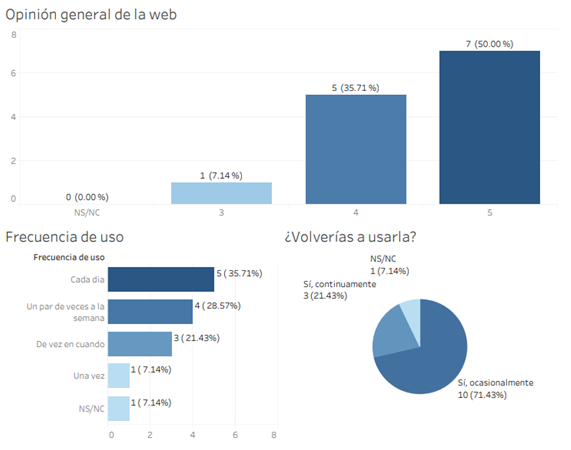
\includegraphics[width=12cm]{Figure_2_3_aireGuruSurveyResults}
   \caption{Aire Guru. Survey results}
\end{figure}

\begin{center}
   \bf Figure 2.3. Aire Guru. Survey results\\
   \end{center}